\documentclass[12pt]{article}
\usepackage{rocca-homework}
\usepackage{graphicx}

\begin{document}

\begin{center}
	\textbf{CS 215 Homework 3} \\
	\textbf{Lucas Vas} \\
	\textbf{09/29/2024}
\end{center}

\subsection*{Problem 1A}
Representing the function F as POS and SOP:
\begin{equation*}
	\begin{split}
		POS & = \bar{A}(\bar{B}\bar{C} + BC) + A(\bar{B}C + B\bar{C})     \\
		SOP & = \bar{A}\bar{B}\bar{C} + \bar{A}BC + A\bar{B}C + AB\bar{C}
	\end{split}
\end{equation*}

\subsection*{Problem 1B}
Gate-level logic circuits for each of the representations.

Product of Sums:

\begin{center}
	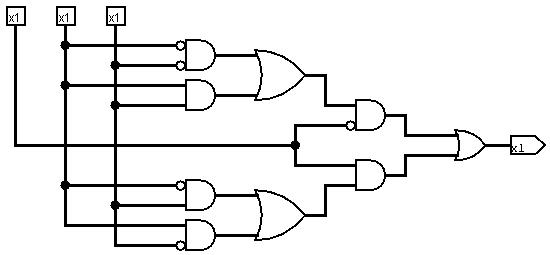
\includegraphics[width=8cm]{cs215_hw3_pos.jpg}
\end{center}

Sum of Products:

\begin{center}
	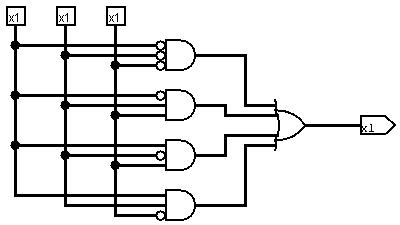
\includegraphics[width=8cm]{cs215_hw3_sop.jpg}
\end{center}

\subsection*{Problem 1C}
Truth table for the function's SOP and POS representations:

\begin{center}
	\begin{tabular}{| c c c | c c |}
		\hline
		A & B & C & SOP & POS \\
		\hline\hline
		0 & 0 & 0 & 1   & 1   \\
		\hline
		0 & 0 & 1 & 0   & 0   \\
		\hline
		0 & 1 & 0 & 0   & 0   \\
		\hline
		0 & 1 & 1 & 1   & 1   \\
		\hline
		1 & 0 & 0 & 0   & 0   \\
		\hline
		1 & 0 & 1 & 1   & 1   \\
		\hline
		1 & 1 & 0 & 1   & 1   \\
		\hline
		1 & 1 & 1 & 0   & 0   \\
		\hline
	\end{tabular}
\end{center}

\subsection*{Problem 2 - Optimization of Circuit}
This is the function form of the circuit:
\begin{equation*}
	F = \bar{A}\bar{B}C + \bar{A}B\bar{C} + \bar{A}BC + A\bar{B}C
\end{equation*}
We'll use a Quine-McCluskey table to simplify the function:
\begin{center}
	\begin{tabular}{| c | c |}
		\hline
		\textbf{Term}     & \textbf{Matched?} \\
		\hline\hline
		$\bar{A}\bar{B}C$ & Yes               \\
		$\bar{A}B\bar{C}$ & Yes               \\
		\hline
		$\bar{A}BC$       & No                \\
		$A\bar{B}C$       & No                \\
		\hline
	\end{tabular}
\end{center}

Matched terms are like so:

\begin{equation*}
	\begin{split}
		\bar{A}\bar{B}C + \bar{A}BC & = \bar{A}C \\
		\bar{A}\bar{B}C + A\bar{B}C & = \bar{B}C \\
		\bar{A}B\bar{C} + \bar{A}BC & = \bar{A}B
	\end{split}
\end{equation*}

The table for this function then becomes:

\begin{center}
	\begin{tabular}{| c | c c c c |}
		\hline
		                    & \textbf{$\bar{A}\bar{B}C$} & \textbf{$\bar{A}B\bar{C}$} & \textbf{$\bar{A}BC$} & \textbf{$A\bar{B}C$} \\
		\hline
		\textbf{$\bar{A}C$} & x                          &                            & x                    &                      \\
		\textbf{$\bar{B}C$} & x                          &                            &                      & x                    \\
		\textbf{$\bar{A}B$} &                            & x                          & x                    &                      \\
		\hline
	\end{tabular}
\end{center}

Therefore, the simplified function is $\bar{A}B + \bar{B}C$, which can be represented as a gate-level circuit as follows:

\begin{center}
	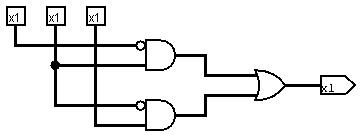
\includegraphics[width=8cm]{cs215_hw3_optimized.jpg}
\end{center}

\end{document}
